\documentclass[12pt,a4paper]{article}
\usepackage[utf8]{inputenc}
\usepackage[spanish]{babel}
\usepackage{amsmath}
\usepackage{amsfonts}
\usepackage{amssymb}
\usepackage{graphicx}
\usepackage{booktabs}
\usepackage{float}
\usepackage{listings}
\usepackage{xcolor}
\usepackage{geometry}
\usepackage{hyperref}
\usepackage{enumitem}

\geometry{margin=2.5cm}

% Configuración para código Python
\lstset{
    language=Python,
    basicstyle=\ttfamily\small,
    keywordstyle=\color{blue},
    commentstyle=\color{green!60!black},
    stringstyle=\color{red},
    numbers=left,
    numberstyle=\tiny,
    stepnumber=1,
    numbersep=5pt,
    backgroundcolor=\color{gray!10},
    showspaces=false,
    showstringspaces=false,
    showtabs=false,
    frame=single,
    tabsize=2,
    captionpos=b,
    breaklines=true,
    breakatwhitespace=false,
    escapeinside={\%*}{*)}
}

\title{\textbf{Problema de las 8 Reinas: Análisis Comparativo de Algoritmos CSP}}
\author{Pola Escobar, José Salazar}
\date{Septiembre 22, 2025}

\begin{document}

\maketitle

\section{Introducción}

El problema de las 8 reinas es un clásico problema de satisfacción de restricciones (CSP) que consiste en colocar 8 reinas en un tablero de ajedrez de 8×8 de modo que ninguna de ellas se ataque entre sí. Este problema ha sido ampliamente estudiado en el campo de la inteligencia artificial como un ejemplo paradigmático para evaluar diferentes técnicas de resolución de CSPs.

\section{Formulación como CSP}

\subsection{Definición del Problema}

El problema de las N reinas se puede formular como un CSP de la siguiente manera:

\subsubsection{Variables}
Cada columna del tablero representa una variable:
$$X = \{X_1, X_2, \ldots, X_N\}$$
donde $X_i$ indica la fila en la que se coloca la reina de la columna $i$.

\subsubsection{Dominios}
Cada reina puede colocarse en cualquier fila:
$$D_i = \{1, 2, \ldots, N\} \quad \forall i \in \{1, 2, \ldots, N\}$$

\subsubsection{Restricciones}
El problema tiene dos tipos de restricciones:

\begin{enumerate}[label=\arabic*.]
    \item \textbf{No puede haber dos reinas en la misma fila:}
    $$X_i \neq X_j \quad \forall i \neq j$$
    
    \item \textbf{No puede haber dos reinas en la misma diagonal:}
    $$|X_i - X_j| \neq |i - j| \quad \forall i \neq j$$
\end{enumerate}

\section{Implementaciones}

Se implementaron tres algoritmos diferentes para resolver el problema:

\subsection{Backtracking Básico}

El algoritmo de backtracking básico explora el espacio de soluciones de manera sistemática, asignando valores a las variables una por una y retrocediendo cuando se detecta una violación de restricciones.

\begin{lstlisting}[caption=Implementación de Backtracking Básico]
def backtracking(tablero, fila, recursive_call, backtrack):
    if fila == len(tablero):
        return tablero, recursive_call, backtrack 
    
    for i in range(len(tablero)):
        if es_valido(tablero, fila, i):
            tablero[fila][i] = 1
            resultado, recursive_call, backtrack = backtracking(
                tablero, fila + 1, recursive_call + 1, backtrack)
            if resultado:
                return resultado, recursive_call, backtrack
            tablero[fila][i] = 0
            backtrack += 1
    return None, recursive_call, backtrack
\end{lstlisting}

\subsection{Forward Checking}

El forward checking mejora el backtracking básico propagando las restricciones hacia adelante, eliminando valores del dominio de variables no asignadas que son inconsistentes con la asignación actual.

\begin{lstlisting}[caption=Implementación de Forward Checking]
def forward_checking(tablero, fila, dominios, recursive_call, backtrack):
    n = len(tablero)
    if fila == n:
        return tablero, recursive_call, backtrack

    for col in dominios[fila][:]:
        tablero[fila][col] = 1
        nuevos = {f: list(dominios[f]) for f in dominios}
        
        # Propagacion de restricciones
        for f in range(fila + 1, n):
            if col in nuevos[f]:
                nuevos[f].remove(col)
            diag1 = col + (f - fila)
            diag2 = col - (f - fila)
            if diag1 in nuevos[f]:
                nuevos[f].remove(diag1)
            if diag2 in nuevos[f]:
                nuevos[f].remove(diag2) 

        if any(len(nuevos[f]) == 0 for f in range(fila + 1, n)):
            tablero[fila][col] = 0
            backtrack += 1
            continue

        resultado, recursive_call, backtrack = forward_checking(
            tablero, fila+1, nuevos, recursive_call + 1, backtrack)
        if resultado: 
            return resultado, recursive_call, backtrack

        tablero[fila][col] = 0
        backtrack += 1

    return None, recursive_call, backtrack
\end{lstlisting}

\subsection{Forward Checking con MRV}

La heurística MRV (Minimum Remaining Values) selecciona la variable con el menor número de valores válidos restantes en su dominio, lo que puede reducir significativamente el espacio de búsqueda.

\begin{lstlisting}[caption=Implementación de Forward Checking con MRV]
def forward_checking_MRV(tablero, dominios, restantes, recursive_call, backtrack):
    if not restantes:
        return [row[:] for row in tablero], recursive_call, backtrack

    # Seleccion MRV: variable con menor dominio
    fila = min(restantes, key=lambda x: len(dominios[x]))
        
    for col in dominios[fila][:]:
        tablero[fila][col] = 1
        nuevos = {f: list(dominios[f]) for f in dominios}
        
        # Propagacion de restricciones
        for f in restantes - {fila}:
            if col in nuevos[f]:
                nuevos[f].remove(col)
            diag1 = col + (f - fila)
            diag2 = col - (f - fila)
            if diag1 in nuevos[f]:
                nuevos[f].remove(diag1)
            if diag2 in nuevos[f]:
                nuevos[f].remove(diag2) 

        if any(len(nuevos[f]) == 0 for f in restantes - {fila}):
            tablero[fila][col] = 0
            backtrack += 1
            continue

        resultado, recursive_call, backtrack = forward_checking_MRV(
            tablero, nuevos, restantes - {fila}, recursive_call + 1, backtrack)
        if resultado: 
            return resultado, recursive_call, backtrack

        tablero[fila][col] = 0
        backtrack += 1

    return None, recursive_call, backtrack
\end{lstlisting}

\section{Experimentos y Resultados}

\subsection{Configuración Experimental}

Se realizaron experimentos con las siguientes configuraciones:
\begin{itemize}
    \item Tamaños de tablero: N = 8, 10, 12, 14, 16, 18, 20
    \item Repeticiones por algoritmo: 4
    \item Métricas evaluadas: tiempo de ejecución, llamadas recursivas, número de backtracks
\end{itemize}

\subsection{Resultados Experimentales}

Los experimentos se ejecutaron de forma paralela para optimizar el tiempo de cómputo. A continuación se presentan los resultados obtenidos:

\subsubsection{Tiempo de Ejecución}

La Figura \ref{fig:tiempo} muestra la evolución del tiempo de ejecución para los tres algoritmos según el tamaño del tablero.

\begin{figure}[H]
\centering
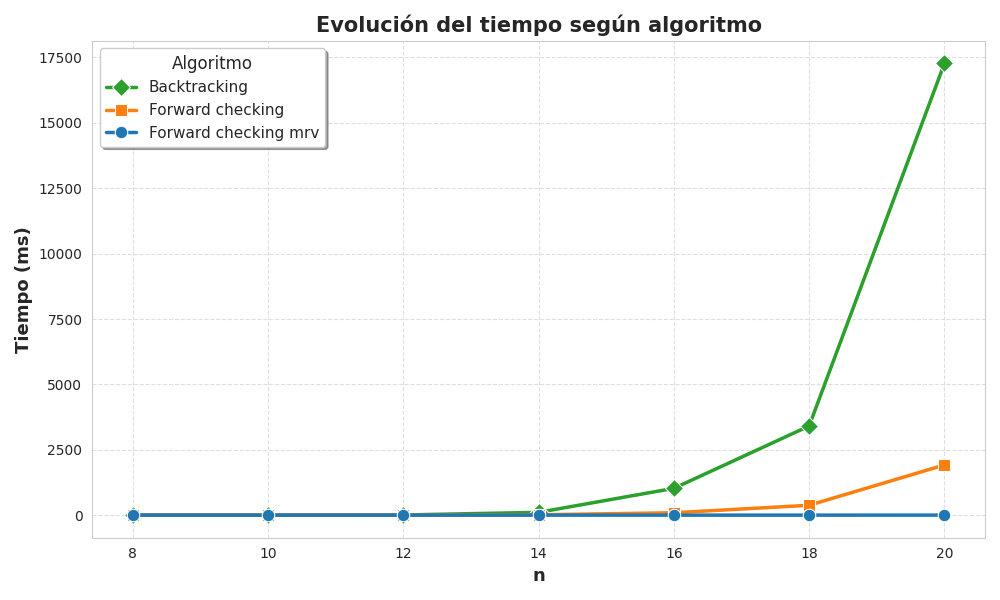
\includegraphics[width=0.8\textwidth]{plots/tiempo_vs_n.png}
\caption{Evolución del tiempo de ejecución según algoritmo}
\label{fig:tiempo}
\end{figure}

\subsubsection{Llamadas Recursivas}

La Figura \ref{fig:llamadas} presenta el número de llamadas recursivas realizadas por cada algoritmo.

\begin{figure}[H]
\centering
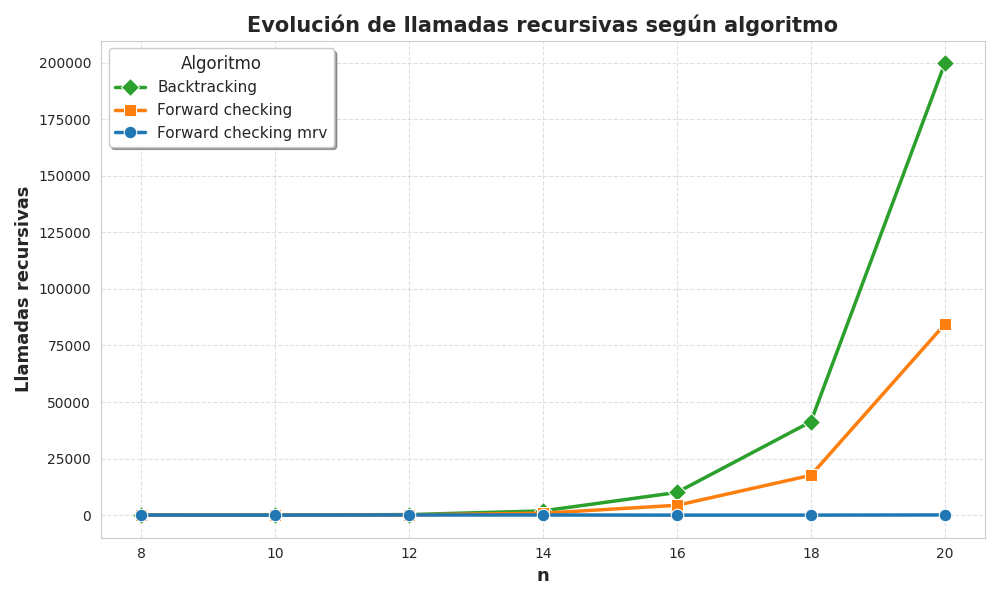
\includegraphics[width=0.8\textwidth]{plots/llamadas_vs_n.png}
\caption{Evolución de llamadas recursivas según algoritmo}
\label{fig:llamadas}
\end{figure}

\subsubsection{Número de Backtracks}

La Figura \ref{fig:backtracks} muestra el número de retrocesos realizados por cada algoritmo.

\begin{figure}[H]
\centering
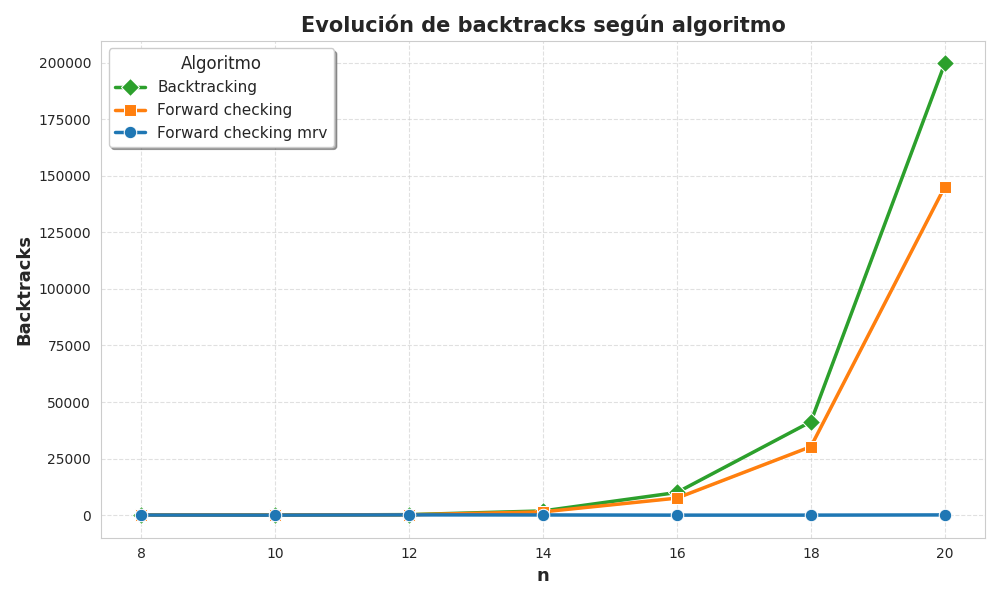
\includegraphics[width=0.8\textwidth]{plots/backtracks_vs_n.png}
\caption{Evolución de backtracks según algoritmo}
\label{fig:backtracks}
\end{figure}

\subsection{Análisis Comparativo}

Basándose en los resultados experimentales, se pueden hacer las siguientes observaciones:

\begin{enumerate}
    \item \textbf{Forward Checking con MRV} es el algoritmo más eficiente en términos de tiempo de ejecución y número de llamadas recursivas.
    
    \item \textbf{Forward Checking} sin MRV muestra mejoras significativas sobre el backtracking básico, especialmente para tableros más grandes.
    
    \item \textbf{Backtracking básico} es el menos eficiente, requiriendo más tiempo y más exploración del espacio de soluciones.
    
    \item La diferencia de rendimiento se acentúa conforme aumenta el tamaño del tablero, demostrando la escalabilidad de las técnicas más avanzadas.
\end{enumerate}

\section{Análisis de Escalabilidad}

Para evaluar la escalabilidad de las técnicas implementadas, se probaron tableros de diferentes tamaños (N = 8, 10, 12, 14, 16, 18, 20). Los resultados muestran que:

\begin{itemize}
    \item El crecimiento del tiempo de ejecución es exponencial para todos los algoritmos, como se esperaba para un problema NP-completo.
    \item Forward Checking con MRV mantiene la mejor relación tiempo/tamaño del tablero.
    \item La diferencia de rendimiento entre algoritmos se amplifica con el aumento del tamaño del tablero.
\end{itemize}

\section{Conclusiones}

\subsection{Reflexión sobre Eficiencia}

Los resultados experimentales confirman que \textbf{Forward Checking con MRV} es la técnica más eficiente para resolver el problema de las N reinas. Esta superioridad se debe a:

\begin{enumerate}
    \item \textbf{Propagación temprana de restricciones}: El forward checking elimina valores inconsistentes antes de explorar ramas del árbol de búsqueda.
    
    \item \textbf{Selección inteligente de variables}: La heurística MRV reduce el factor de ramificación del árbol de búsqueda.
    
    \item \textbf{Detección temprana de fallos}: La combinación de ambas técnicas permite detectar inconsistencias más rápidamente.
\end{enumerate}

\subsection{Lecciones Aprendidas}

\begin{itemize}
    \item La propagación de restricciones es crucial para mejorar la eficiencia de los algoritmos CSP.
    \item Las heurísticas de selección de variables pueden tener un impacto significativo en el rendimiento.
    \item La combinación de múltiples técnicas de optimización puede producir mejoras sinérgicas.
    \item La medición empírica es esencial para validar las mejoras teóricas.
\end{itemize}

\section{Código Fuente}

El código fuente completo del proyecto está disponible en el archivo \texttt{ochoreinas.py}, que incluye:

\begin{itemize}
    \item Implementación de los tres algoritmos
    \item Sistema de logging para monitoreo
    \item Ejecución paralela de experimentos
    \item Generación automática de gráficos
    \item Exportación de resultados a CSV
\end{itemize}

\section{Referencias}

\begin{enumerate}
    \item Russell, S., \& Norvig, P. (2020). \textit{Artificial Intelligence: A Modern Approach}. 4th Edition. Pearson.
    \item Dechter, R. (2003). \textit{Constraint Processing}. Morgan Kaufmann.
    \item Mackworth, A. K. (1977). Consistency in networks of relations. \textit{Artificial Intelligence}, 8(1), 99-118.
\end{enumerate}

\end{document}
